\input{../header.tex}

\subject{VERSUCH NUMMER 701}
\title{Reichweite von Alphastrahlung}
\date{
  Durchführung: 11.04.2023
  \hspace{3em}
  Abgabe: 18.04.2023
}

\begin{document}

\maketitle
\thispagestyle{empty}
\tableofcontents
\newpage
\setcounter{page}{1}
\section{Ziel}
\label{sec:Ziel}

In diesem Versuch soll die Reichweite von Alphastrahlung sowie die Statistik des radioaktiven
Zerfalls eines Am-Präparats untersucht werden.
\section{Theorie}
\label{sec:Theorie}

Durch die Messung der Reichweite von Alphastrahlung kann auch dessen
Energie bestimmt werden. Durch Anregung und Dissoziation von Molekülen beim 
Durchlaufen eines Materials verliert die Alphastrahlung an Energie. Dieser
Energieverlust ist abhängig von der Energie der Alphastrahlung sowie der
Dichte des durchlaufenen Materials und berechnet sich über die Bethe-Bloch-Gleichung
\begin{equation}
    -\frac{d E_\alpha}{d x}=\frac{z^2 e^4}{4 \pi \epsilon_0 m_e} \frac{n Z}{v^2} \ln \left(\frac{2 m_e v^2}{I}\right) \; .
    \label{eqn: energieverlust}
\end{equation}
Dabei ist $z$ die Ladung und $v$ die Geschwindigkeit der Alphastrahlung; $Z$ die Ordnungszahl,
$n$ die Teilchendichte und $I$ die Ionisierungsenergie des Targetgases. 

Die Reichweite $R$ ist die Strecke bis zur vollständigen Abbremsung eines 
Alphateilchens und berechnet sich durch 
\begin{equation*}
    R=\int_0^{E_\alpha} \frac{d E_\alpha}{-d E_\alpha / d x} \; .
\end{equation*}
Bei kleinen Energien nehmen Ladungsaustauschprozesse stark zu und der
Energieverlust lässt sich nicht mehr durch die Bethe-Bloch-Gleichung 
\eqref{eqn: energieverlust} beschreiben. Stattdessen nutzt man zur Bestimmung
der mittleren Reichweite $R_{\symup{m}}$ empirisch bestimmte Kurven. Für 
Energien $E_{\symup{\alpha}} \leq 2.5 \, \unit{\MeV}$ lässt sich die mittlere 
Reichweite über $R_{\symup{m}} = 3.1 \cdot E_{\symup{\alpha}}^{3/2}$ bestimmen.

In Gasen ist die Reichweite der Alphastrahlung proportional zum Druck und kann
über eine Absorptionsmessung bestimmt werden, bei der der Druck variiert wird.
Für die effektive Länge gilt dann 
\begin{equation}
    x = x_0 \frac{p}{p_0} \, .
    \label{eqn:effLaeng}
\end{equation}
Dabei ist $x_0$ der Abstand zwischen dem Detektor und dem Alphastrahler. 
$p_0$ ist der Normaldruck $p_0 = 1013 \, \symup{mbar}$.
\section{Vorbereitungsaufgaben}
\label{sec:vorbereitung}

Ein Halbleiterzähler besteht aus je einem Halbleiter mit n-Leitung und p-Leitung. An der Kontaktstelle entsteht durch Diffusion eine Zone mit
beweglichen Ladungsträgern. Dies passiert solange bis das so aufgebaute elektrische Feld die weitere Diffusion verhindert. Der Übergang zwischen 
den Halbleitern ähnelt einer Diode. Wenn nun der n-Bereich mit einer Anode und der p-Bereich mit einer Kathode verbunden wird, vergrößert sich
der Bereich der freien Ladungsträger. Dieser Bereich wird auch Sperrzone genannt.

Wenn ein ionisierendes Teilchen durch diese Zone durchdringt, werden Elektronen und Löcher erzeugt. dadurch entsteht ein kurzzeitiger Stromfluss,
der messbar ist.
\section{Aufbau}
\label{sec:Aufbau}
Für die Messung der Reichweite von $\alpha$-Strahlen wird der in \autoref{fig:Aufbau} gezeigte Versuchsaufbau verwendet.
Die benötigten Bauteile sind eine Vakuumpummpe inklusive Druckmessgerät und Ventil, ein Vielkanalanalysator, einen luftdichten Glaszylinder mit Skala zur ABstandsmessung,
den Alphastrahler, einen in \autoref{sec:vorbereitung} beschriebenen Halbleiter-Detektor und einen Vorverstärker.
\begin{figure}
    \centering
    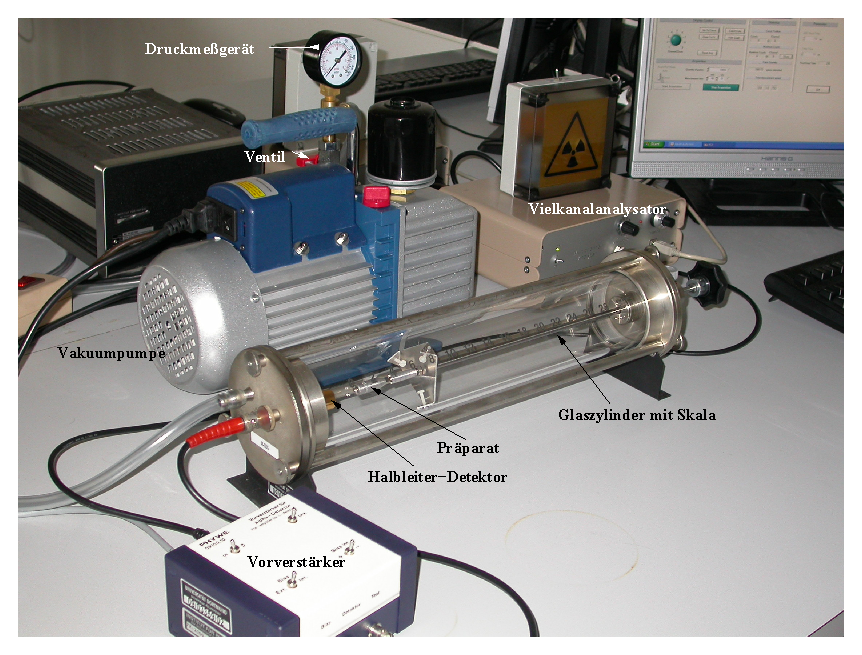
\includegraphics[height = 6cm]{Aufbau.pdf}
    \caption{Aufbau zur Messung der Reichweite von $\alpha$-Strahlen \cite{ap701}.}
    \label{fig:Aufbau}
\end{figure}
Die Bauteile werden ordnungsgemäß angeschlossen und die Messung kann Beginnen.

\section{Durchführung}
\label{sec:Durchführung}

Zunächst wird die Probe auf einen festen Abstand eingestellt und  die Kammer mithilfe der Vakuumpumpe evakuiert.
Wenn die Kammer einen Druck von $0\,\text{m}\unit{\bar}$ wird das Messprogramm auf dem Computer gestartet und die Messung beginnt. 
In den 2 Minuten die jede Messung durchgeführt wird, misst das Programm die Häufigkeit der Energien, die die Helium-Kerne besessen haben und hat als Ausgabe werden die Anzahl der 
detektierten $\alpha$-Teilchen, die häufigste Energie derer und die Häufigkeit dieser angezeigt.
Nach der Messung in der evakuierten Kammer wird der Druck in der Kammer auf $50\, \text{m}\unit{\bar}$ erhöht und ein erneuter Messdurchlauf gestartet.
Die Messung wird so lange fortgesetzt bis entweder ein Druck von $p= 1\, \unit{\bar}$ (welcher dem atmosphärischen Druck entspricht) erreicht ist oder keine Teilchen mehr nachgewiesen werden können.
Insgesamt werden so zwei Abstände ausgemessen.
Im Anschluss dazu wird dei Statistik des radioaktiven Zerfalls untersucht.
Hierzu werden Druck, Temperatur und Abstand konstant gehalten und die Messung 100-mal wiederholt.
Gemessen wird 10 $\unit{\second}$ lang.
Es werden jeweils die Anzahl der detektierten Teilchen notiert, um später eine Aussage über die stochastische Verteilung der Häufigkeit von Zerfällen treffen zu können.

\section{Auswertung}
\label{sec:Auswertung}

\input{fehlerrechnung.tex}

\subsection{Reichweite von Alphastrahlung}

\begin{table}
    \centering
    \caption{Druckabhängigkeit der Zählrate, der Energie und der effektiven Länge bei einem Abstand zwischen Probe und Detektor von $x_0 = 3\,\unit{\cm}$.}
\begin{tabular}{c c c c c}
    \toprule
    $p \mathbin{/}\unit{\mbar}$ &Zählrate& Energie & Zählrate des Maximums & $x \mathbin{/}\unit{\m}$ \\
    \midrule
                                     0&55341&831&190&0.0000 \\
                           50&54428&816&195&0.0015 \\
                           100&53962&791&201&0.0030 \\
                         150&53946&775&213&0.0044 \\
                         200&52866&715&234&0.0059 \\
                         250&52531&663&234&0.0074 \\
                         300&51795&615&242&0.0089 \\
                         350&51292&611&263&0.0104 \\
                         400&50646&583&252&0.0118 \\
                         450&49603&547&256&0.0133 \\
                         500&48743&527&276&0.0148 \\
                         550&47524&492&261&0.0163 \\
                         600&45813&431&268&0.0178 \\
                         650&42665&371&278&0.0192 \\
                         700&36549&348&283&0.0207 \\
                         750&24399&271&288&0.0222 \\
                         800&15029&262&256&0.0237 \\
                           850&3142&97&262&0.0252 \\
                              900&92&6&262&0.0267 \\
                              950&10&1&274&0.0281 \\
                              1000&1&1&259&0.0296 \\
    \bottomrule
    \end{tabular}
    \label{tab:3cm}
\end{table}
\section{Diskussion}
\label{sec:Diskussion}
Da es keine theoretischen Werte als Referenz bzw. Vergleich gibt, bleibt ein Begründen und Abwiegen möglicher Fehler und 
Messunsicherheiten weitestgehend aus.
Einzig und allein kann über die Unsicherheit bei der Geraden zur Bestimmung des Energieverlustes diskutiert werden,
da die Steigung stark davon abhängt, welche Werte man mit in die Berechnung einfließen lässt und welche man auslässt.
Der übergang verlief fließend, sodass es hier zu Abweichungen kommen kann.
Auch beim Ablesen des Manometer ist ein gewisser Fehler nicht auszuschließen. Weitere Messunsicherheiten sind durch das Verwenden eines 
Computerprogramms auf ein Minimum reduziert worden.

\newpage
\printbibliography
\nocite{ap308}
\nocite{matplotlib}
\nocite{numpy}
\nocite{scipy}
\nocite{uncertainties}
\nocite{reback2020pandas}

\newpage
%\includepdf[scale=0.9,pages=1,pagecommand=\section*{Anhang}\thispagestyle{empty}]{messdaten.pdf}
%\addcontentsline{toc}{section}{\protect\numberline{}Anhang}
%\includepdf[scale=0.9,pages=2-]{messdaten.pdf}
%\includepdf[pages=-]{messdaten.pdf}

\end{document}
